\important{Focus sur: l'éolienne}

\begin{center}
    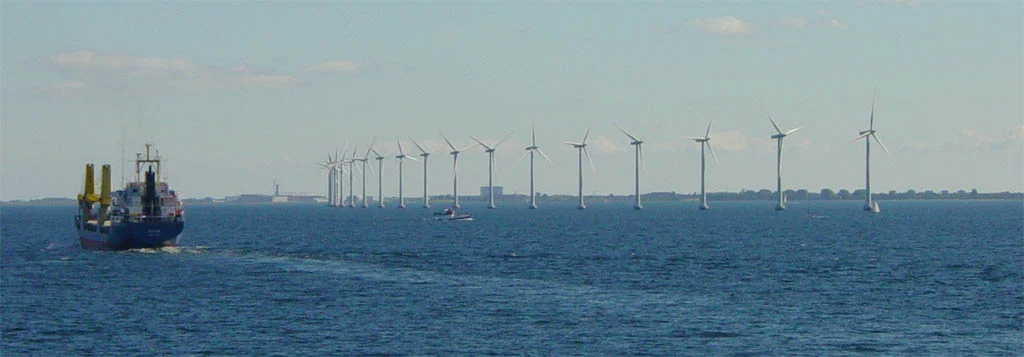
\includegraphics[width=8cm]{images/eoliennes.png}

    \textit{Champ d'éoliennes au large de Copenhague (Danemark)}
\end{center}


Une éolienne est un dispositif qui permet de produire de l'électricité à partir du vent. Elle est composée de grandes pales situées au sommet d'un pylone.
Quand le vent souffle, il fait tourner les pales. Ce mouvement de rotation entraîne un alternateur qui produit de l'électricité.
Pour produire beaucoup d'électricité, on installe souvent plusieurs dizaines d'éoliennes au même endroit : c'est ce qu'on appelle un parc éolien.

L'éolienne utilise le vent, une source d'énergie renouvelable, et ne rejette pas de CO\textsubscript{2}. La production d'électricité dépend du vent : elle est irrégulière et impossible à prévoir précisément.
Une éolienne peut être gênante pour les habitants proches (bruit, impact visuel sur le paysage) et dangereuse pour certains oiseaux.